\section{Methodology}
\label{sec:method}

In this section, we present the computational strategy used for computing the
active subspace in the case of H$_2$/O$_2$ reaction kinetics with uncertain
pre-exponent of individual reaction rates provided in Table~\ref{tab:kinetics}.
Specifically, we employ two strategies: 
A gradient-based strategy that involves computation of model
gradients in order to construct the matrix $\hat{\mat{C}}$
in~\eqref{eq:chat}, and a gradient-free approach 
that involves a (\alennote{should we say 
regression-based?}) local linear approximation of
the model output to circumvent the computational cost associated with gradient
computation. The gradient-based approach is based on Algorithm
1.1, and the gradient-free approach is based on Algorithm 1.2
in~\cite{Constantine:2015}. In this work, we implement the two
strategies in an iterative manner and demonstrate potential for
additional savings in both cases.  For the present application,
our findings based on the two strategies are observed to be consistent.  
Since,
the gradient-free approach is more efficient, this observation
encourages its use for high-dimensional applications as discussed later in
Section~\ref{sec:app}. 
%Note however, that the model output is required to be
%differentiable throughout the input domain in both cases.

\subsection{Gradient-based approach}
\label{sub:grad}

As discussed earlier, in the gradient-based approach, the elements of
$\hat{\mat{C}}$ are estimated using model gradients.  In situations where the
gradient is not available analytically, one could consider using finite
difference and other relatively more efficient techniques such as automatic
differentiation~\cite{Kiparissides:2009} and adjoint-based gradient
computation~\cite{Jameson:1988,Gunzburger:2003,Borzi:2011,Alexanderian:2017}.
Model evaluations at neighbouring points are required if finite difference is
used. Hence, for $N$ samples in a $d$-dimensional parameter space, $N(d+1)$
model evaluations are needed. 

We begin by evaluating the gradient of the model output, $\nabla_{\bm{\xi}}f$,
at an initial set of $n_1$ samples.  For this purpose, $\bm{\xi}_i$'s are
projected to the physical space as $\bm{\theta}_i$'s. 
\alennote{The mention of $\bm{\theta}$ is redundant. 
Say what $\bm{\xi}_i$, $i = 1, \ldots, n_1$ are before using them.} 
Using the gradient
evaluations, the matrix, $\hat{\mat{C}}$ is computed. Eigenvalue decomposition
of $\hat{\mat{C}}$ yields an initial estimate of the dominant eigenspace,
$\hat{\mat{W}}_1$ and corresponding set of eigenvalues,
$\hat{\mat{\Lambda}}_1$.  At each subsequent iteration, model evaluations are
generated at a new set of $n_s$ samples. The new set of gradient evaluations
are augmented with the available set to re-construct $\hat{\mat{C}}$ followed
by its eigenvalue decomposition. The relative change in the norm of the
difference in squared value of individual components of the dominant
eigenvectors between subsequent iterations is evaluated. The process is
terminated and the resulting eigenspace is considered to be converged once
highest relative change at iteration $k$, $\delta \hat{\mat{W}}_{1,j}^{(k)}$,
is smaller than a given tolerance, $\tau$.  A regression fit to
$G(\hat{\mat{W}}_1^\top\bm{\xi})$ is used as a surrogate to characterize and
quantify the uncertainty in the model output. Moreover, the components of the
dominant eigenvectors are used to compute the activity scores, $\bm{\nu}_r(f)$,
which provide insight into the relative importance of the uncertain inputs.
Note that the index, $r$, corresponds to the number of dominant eigenvectors in
$\hat{\mat{W}}_1$. The sequence of steps for the gradient-based approach are
provided in Algorithm~\ref{alg:grad}.

%% Grad-based algorithm

\bigskip
\begin{breakablealgorithm}
\renewcommand{\algorithmicrequire}{\textbf{Input:}}
\renewcommand{\algorithmicensure}{\textbf{Output:}}
  \caption{An iterative gradient-based approach for discovering the active subspace}
  \begin{algorithmic}[1]
\Require $\theta_l$, $\theta_u$, $\tau$. 
\Ensure $\hat{\mat{\Lambda}}$, $\hat{\mat{W}}$, $\bm{\nu}_r(f)$ %$\eta$. %
    \Procedure{Gradient-based}{}
    \State Set $k$ = 0
	\State Draw $n_k$ random samples, $\{\bm{\xi}_i\}_{i=1}^{n_k}$ 
         according to $\pi_{\bm{\xi}}$. 
    \State Set $N_\text{total}$ = $n_k$ 
	\iffalse \State Project to the physical space:
        $\{\bm{\theta}_k\}_{k=1}^{n_r}=\theta_l+0.5(\theta_u-\theta_l)\{\bm{\xi}_k\}_{k=1}^{n_r}$ \fi
	\State For each $i=1, \ldots, N_\text{total}$, compute $f(\bm{\xi}_i)$ and the gradient $\bm{g}^i = \nabla_{\bm{\xi}}f(\bm{\xi}_i)$
    \iffalse  
	\Statex\hspace{5mm} Using Finite Difference: 
	\Statex\hspace{5mm} i. Assign a small increment, $d\xi$.
	\Statex\hspace{5mm} ii. Augment the set of samples with neighboring points.
	\be \{\bm{\Xi}_k\}_{k=1}^{n_1(N_p+1)}:~\{\bm{\xi}_k\}_{k=1}^{n_1} \cup
        \{\xi_{k,j}+d\xi\}_{j=1}^{N_p} \nonumber
	\ee
	\Statex\hspace{5mm} iii. Project to the physical space:
        $\{\bm{\theta}_k\}_{k=1}^{n_1(N_p+1)}=\theta_l+0.5(\theta_u-\theta_l)\{\bm{\Xi}_k\}_{k=1}^{n_1(N_p+1)}$
	\Statex\hspace{5mm} iv. Using the augmented set, $\{\bm{\theta}_k\}_{k=1}^{n_1(N_p+1)}$
         compute $\bm{g}^i$.
         \fi 
	\State Compute $\hat{\mat{C}}$ and its eigenvalue decomposition 
		$\hat{\mat{C}}$= $\frac{1}{N_\text{total}}\sum\limits_{i=1}^{N_\text{total}}[\bm{g}^i][\bm{g}^i]^\top$ = 
		$\hat{\mat{W}}^{(k)}\hat{\mat{\Lambda}}^{(k)} \hat{\mat{W}}^{(k)\top}$
	%\State Eigenvalue decomposition, $\mat{C}$ = $W^{(0)}\Lambda^{(0)} W^{(0)\top}$%
	\State Partition: $\hat{\mat{\Lambda}}^{(k)}=
        \begin{bmatrix} \hat{\mat{\Lambda}}_1^{(k)} & \\ & \hat{\mat{\Lambda}}_2^{(k)} \end{bmatrix}$, 
        $\hat{\mat{W}}^{(k)}=\begin{bmatrix} \hat{\mat{W}}_1^{(k)} & \hat{\mat{W}}_2^{(k)} \end{bmatrix}$, 
        $\hat{\mat{\Lambda}}_1^{(k)}\in \mathbb{R}^{N_p\times r}$
	\Loop
		\State Set $k$ = $k$ + 1
		\State Draw $n_k =  \lceil\beta n_{k-1}\rceil$  new random samples 
                $\{\bm{\xi}_i\}_{i=1}^{n_k}$  $\beta\in[0,1]$  $k = n_{k-1}+1,\ldots,n_{k-1}+n_k$.
                
	%	\State Project $\bm{\xi}_k$~$\rightarrow$~$\bm{\theta}_k$.%
		\State Set $N_\text{total}$ = $N_\text{total}$ + $n_k$ 
		\State Compute $\bm{g}^i = \nabla_{\bm{\xi}_i}f(\bm{\xi}_i)$, 
             	$i=n_{k-1}+1, \ldots, n_{k-1}+n_k$.  
		\State Compute $\hat{\mat{C}}$ = 
        	$\frac{1}{N_\text{total}}\sum\limits_{k=1}^{N_\text{total}}[\bm{g}^i][\bm{g}^i]^\top$
		\State Eigenvalue decomposition, $\hat{\mat{C}}$ = $\hat{\mat{W}}^{(k)}\hat{\mat{\Lambda}}^{(k)}
		 \hat{\mat{W}}^{(k)\top}$
		\State Compute $\delta \hat{\mat{W}}_{1,j}^{(k)}$ = 
                       \scalebox{1.25}{$\frac{\|(\hat{\mat{W}}_{1,j}^{k})^2 - 
                       (\hat{\mat{W}}_{1,j}^{k-1})^2\|}{\|(\hat{\mat{W}}_{1,j}^{k-1})^2\|}$}, 
                       $j = 1,\ldots,r$.
		\If {$\max\left(\delta \hat{\mat{W}}_{1,j}^{(k)}\right)<\tau$}
			\State break
		\EndIf
	\EndLoop
	\State Compute $\nu_{i,r}(f) = \sum\limits_{j=1}^{r} \hat{\mat{\Lambda}}_{i,j}\hat{\mat{W}}_{i,j}^2$,
	$i=1,\ldots,N_p$.
	
    \EndProcedure
  \end{algorithmic}
  \label{alg:grad}
\end{breakablealgorithm}
\bigskip

To motivate our iterative strategy, we implement
Algorithm~\ref{alg:grad} to the 19-dimensional H$_2$/O$_2$ reaction kinetics
problem with uncertain $A_i$'s. For the purpose of verification,
$\hat{\mat{C}}$ is initially constructed using a large set of samples
($N$~=~1000) in the input domain and the corresponding active subspace is
computed. In Figure~\ref{fig:eig_comp}~(left), we illustrate the comparison of
the resulting normalized eigenvalue spectrum ($\lambda_1, \ldots, 
\lambda_{19}$) with the same using a much 
smaller set of samples, $n$~=~$\{20,40,80,120\}$.
Additionally, in Figure~\ref{fig:eig_comp} (right), we compare relative $L_2$
norm of the difference between the first five eigenvectors of $\hat{\mat{C}}$.
\alennote{This last sentence is unclear.}

%
\begin{figure}[htbp]
 \begin{center}
  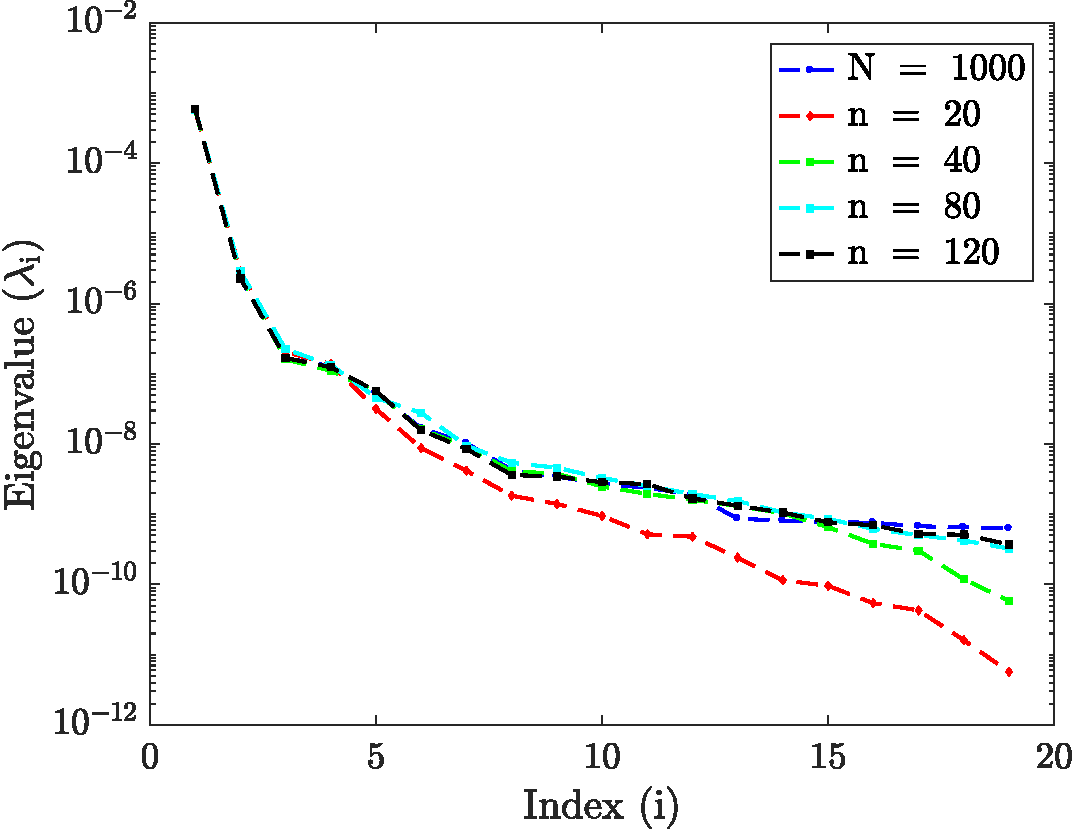
\includegraphics[width=0.45\textwidth]{./Figures/eig_comp}
   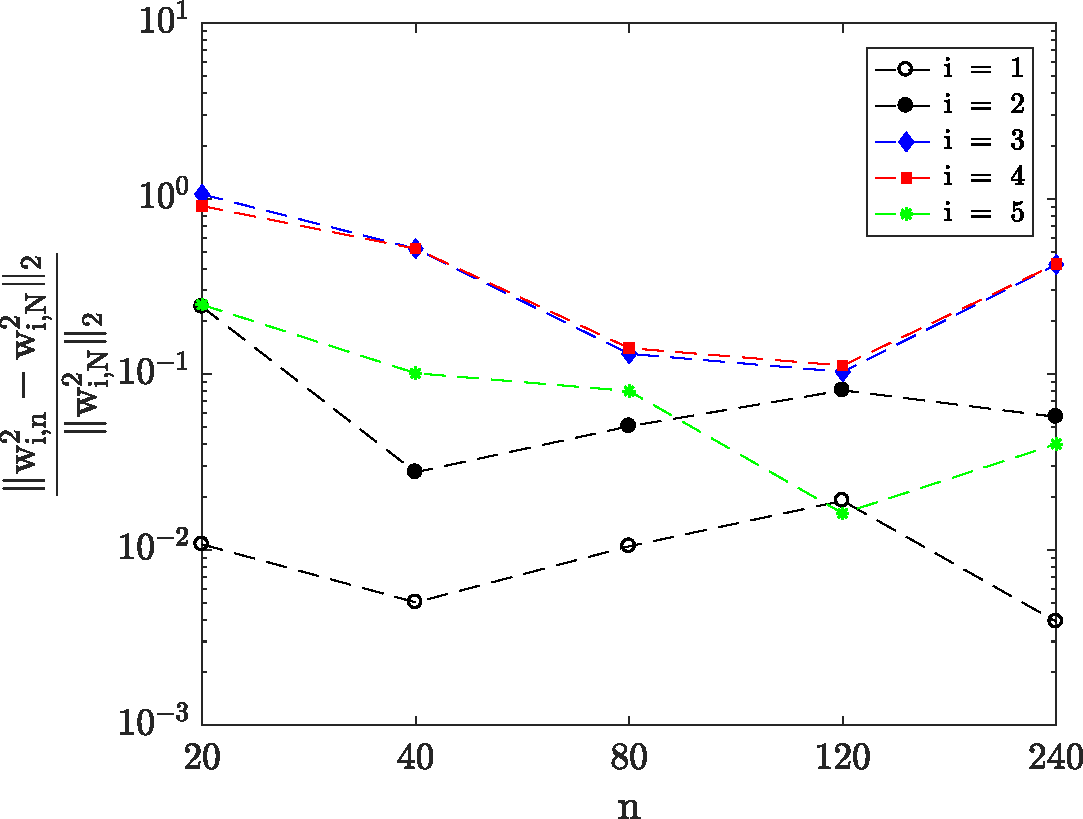
\includegraphics[width=0.48\textwidth]{./Figures/err_eigv_1_5}
\caption{Left: A comparison of the normalized eigenvalue spectrum using $n$ = $\{20,40,80,120\}$ samples with that
obtained using a much larger sample size, $N$~=~1000. Right: Relative $L_2$ 
norm of the difference between
the square of individual components of the first five eigenvectors of $\mat{C}$, constructed using 
$N$~=~1000 samples ($w_{i,N}$), and using a smaller sample size, $n$ ranging from 20 to 240 ($w_{i,n}$).} 
\label{fig:eig_comp}
\end{center}
\end{figure}
%
We observe that the dominant eigenvalues, $\lambda_1, \ldots, \lambda_4$, 
are approximated 
reasonably well with just 20 samples. As expected, the accuracy of higher-order eigenvalues is observed
to improve with the sample size. Similarly, the relative error associated with the dominant eigenvectors
($i$ = 1,2) is found to range from $\mathcal{O}(10^{-2} - 10^{-1})$ and is relatively much smaller than 
the higher-order eigenvectors. In this case, since 
$\left(\frac{\lambda_1}{\lambda_2}\right)\gg 1$, we expect 
a 1-dimensional active subspace. Hence, the first eigenvector 
sufficiently captures the uncertainty in
the  model output. Therefore, a sample size of 20 is adequate for computing the active subspace in this
case. The iterative strategy therefore offers a significant potential for computational advantage. 
However, estimating the gradient of the model output imposes a significant computational burden.
Hence, we next explore the applicability of a so-called gradient-free approach
as mentioned earlier.

\subsection{Gradient-free approach}
\label{sub:gradfree}

\alennote{I don't see the point of this paragraph; part of it that 
explains the gradient-free approach is unclear, and the part 
that seems to motivate its use is something to mention in the introduction.
Just say what the gradient-free approach is about, and say that we 
follow an iterative strategies as before.}
As mentioned earlier, the gradient-free approach does not involve computation
of the gradient of the model output. Instead, a least-squares fit is performed
to the local linear regression-based approximation to the model output. While
the gradient-free approach offers a significant potential for additional
computational savings, its ability to reasonably approximate the active
subspace has not been investigated for a wide variety of
problems~\cite{Constantine:2015}. We are motivated by the
potential of this approach in reducing the computational effort
associated with the active subspace computation. Moreover, this effort could
help advance this approach and further motivate its usage for a wide variety of
high-dimensional applications in the future. 

First, we implement the gradient-free approach to the 19-dimensional problem and compare our findings with
those obtained using the gradient-based approach. Later, in
Section~\ref{sec:app}, we compute the active subspace for a 33-dimensional application using the gradient-free
approach. Once again, the strategy is implemented in an iterative manner as shown in~\ref{sub:grad}. 
It is observed that the results from the gradient-free approach are consistent with the gradient-based approach
as discussed further below.

In the gradient-free approach, the model output is first computed at an initial set of $n_1$ samples. An independent
set of $M$ samples is also drawn according to the joint probability distribution of the inputs. For each sample
in $M$, $p$ nearest neighbours in the $n_1$ set are identified. A least-squares fit to model evaluations at
the $p$ samples is performed. The slope vector ($\bm{b}_i$) of the regression-fit is stored separately and the process is
repeated for each sample in $M$. The symmetric and positive semi-definite matrix, $\hat{\mat{C}}$ is hence constructed
using the slope vectors as follows:
%
\be
\hat{\mat{C}} = \frac{1}{M}\sum\limits_{i=1}^{M}\bm{b}_i\bm{b}_i^\top = \hat{\bm{W}}\hat{\bm{\Lambda}}\hat{\bm{W}}^\top
\ee
%
Hence, the gradient-free approach essentially differs in the procedure for constructing the matrix, $\hat{\mat{C}}$.
The active subspace computation involves the same sequence of steps as outlined previously for the gradient-based 
approach in Algorithm~\ref{alg:grad}. The procedure for constructing $\hat{\mat{C}}$ using local linear approximation
of the model output is provided in Algorithm~\ref{alg:free2}.

%\bigskip
%\begin{breakablealgorithm}
%\renewcommand{\algorithmicrequire}{\textbf{Input:}}
%\renewcommand{\algorithmicensure}{\textbf{Output:}}
%  \caption{An iterative gradient-free approach for discovering the active subspace}
%  \begin{algorithmic}[1]
%\Require $\theta_l$, $\theta_u$, $M$, $\tau$. 
%\Ensure $\Lambda$, $W$, $\alpha$ %$\eta$. 
%    \Procedure{Gradient-free}{}
%    \State Set $k$ = 0
%	\State Draw $n_k$ random samples, $\{\bm{\xi}_j\}_{j=1}^{n_k}$
%	\State Set $N_\text{total}$ = $n_k$ 
%	\iffalse \State Project to the physical space:
%        $\{\bm{\theta}_k\}_{i=1}^{n_k}=\theta_l+0.5(\theta_u-\theta_l)\{\bm{\xi}_k\}_{k=1}^{n_r}$
%        \fi
%     \State Draw $M$ random samples, $\{\bm{\nu}_i\}_{i=1}^{M}$ 
%	\State Compute $f(\bm\xi_j)$, $j=1, \ldots, N_\text{total}$.
%	\State Compute the matrix $\mathbb{C}$ and its eigenvalue decomposition using Algorithm 3
%	%\State Eigenvalue decomposition, $\mat{C}$ = $W^{(r)}\Lambda^{(r)} W^{(r)\top}$
%	\State Partition: $\Lambda^{(k)}~=~ 
%        \begin{bmatrix} \Lambda_1^{(k)} & \\ & \Lambda_2^{(k)} \end{bmatrix}$, 
%        $W^{(k)}~=~\begin{bmatrix} W_1^{(k)} & W_2^{(k)} \end{bmatrix}$, 
%        $\Lambda_1^{(k)}\in \mathbb{R}^{d\times\mathcal{S}}$
%	\Loop
%		\State Set $k$ = $k$ + 1
%		\State Draw $n_k =  \beta n_{k-1}$  new random samples 
%		$\{\bm{\xi}_j\}_{j=1}^{n_k}$  $\beta =??$  $j = n_{k-1}+1,\ldots,n_{k-1}+n_k$. 
%        \State $N_\text{total}$ = $N_\text{total}$ + $n_k$    
%	\iffalse	\State Project $\bm{\xi}_k$~$\rightarrow$~$\bm{\theta}_k$. \fi
%		 
%		\State Compute $f(\bm\xi_j)$, $j=n_{k-1}+1, \ldots, n_{k-1}+n_k$.  
%		\State Construct the matrix, $\mat{C}$ and its eigenvalue decomposition
%		\State Compute $\delta W_{1,j}^{(k)}$ = 
%                       \scalebox{1.25}{$\frac{\|(W_{1,j}^{k})^2 - 
%                       (W_{1,j}^{k-1})^2\|}{\|(W_{1,j}^{k-1})^2\|}$}, 
%                       $j = 1,\ldots,\mathcal{S}$.
%		\If {$\max\left(\delta W_{1,j}^{(k)}\right)<\tau$}
%			\State break
%		\EndIf
%	\EndLoop
%	\State Compute $\alpha_i(N_\text{total}) = \sum\limits_{j=1}^{\mathcal{S}} \Lambda_{1_{i,j}}W_{1_{i,j}}^2$,
%	$i=1,\ldots,d$.
%    \EndProcedure
%  \end{algorithmic}
%  \label{alg:free1}
%\end{breakablealgorithm}
%\bigskip
%
\bigskip
\begin{breakablealgorithm}
\renewcommand{\algorithmicrequire}{\textbf{Input:}}
\renewcommand{\algorithmicensure}{\textbf{Output:}}
  \caption{Algorithm for constructing the matrix, $\mat{C}$}
  \begin{algorithmic}[1]
	\Procedure{Local Linear Approximation}{} 
	\State Draw $N$ random samples, $\{\bm{\xi}_j\}_{j=1}^{N}$ 
	according to $\pi_{\bm{\xi}}$.
	\iffalse \State Project to the physical space:
	$\{\bm{\theta}_k\}_{k=1}^{N}=\theta_l+0.5(\theta_u-\theta_l)\{\bm{\xi}_k\}_{k=1}^{N}$ \fi
	\State Compute $f(\bm\xi_j)$, $j=1, \ldots, N$.
	\State Draw $M$ random samples, $\{\bm{\zeta}_i\}_{i=1}^{M}$
	according to $\pi_{\bm{\xi}}$.
	\State Choose an integer $p \leq N$ 
	\State For each $i=1, \ldots, M$, compute 
	\[
	\begin{aligned}
	\Phi_i &= \{ p \text{ nearest points in } \{\bm{\xi}_j\}_{j=1}^{N} \text{ to } \bm{\zeta}_i\}\\
	\vspace{-2mm}
	\Psi_i &= \text{subset of } f(\bm\xi_j) \text{ corresponding to the points in } \Phi_i
	\end{aligned}
	\]
	\State Compute linear least square fits 
	 $f(\bm\xi_j) \approx c_i + b_i^T\bm{\xi}_j$, \  $\bm{\xi}_j \in \Phi_i, \ f(\bm\xi_j) \in \Psi_i$
	\State Compute the matrix 
	\[
	\hat{\mat{C}} \approx \frac{1}{M} \sum_{i=1}^{M} b_i b_i^T = \hat{\mat{W}}\hat{\mat{\Lambda}}\hat{\mat{W}}^\top
	\]
	\EndProcedure
  \end{algorithmic}
  \label{alg:free2}
\end{breakablealgorithm}
\bigskip


The gradient-free approach when implemented to the 19-dimensional H$_2$/O$_2$ reaction kinetics problem
with uncertain pre-exponents ($A_i$'s) also yielded a 1-dimensional active subspace. In Figure~\ref{fig:comp} (left),
we provide a comparison of the components of the dominant eigenvector, obtained using the two approaches.
Additionally, the quantity, $\delta \hat{\mat{W}}_{1,j}^{(r)}$ is also plotted in
Figure~\ref{fig:comp} (right) to illustrate convergence characteristics for the gradient-free approach.
%
\begin{figure}[htbp]
 \begin{center}
  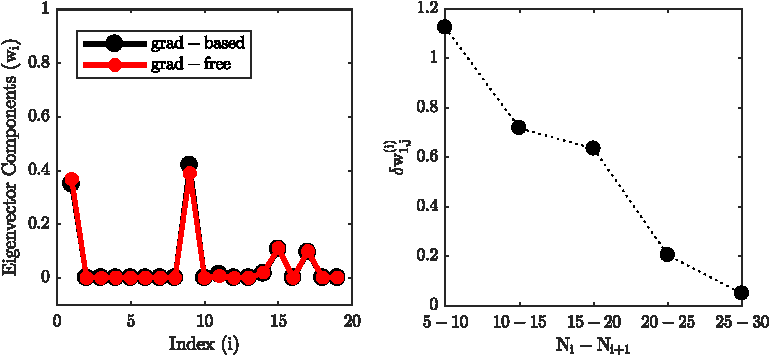
\includegraphics[width=0.8\textwidth]{./Figures/eigv6}
\caption{Left: An illustrative comparison of individual components of the converged dominant eigenvector obtained
using the two approaches discussed in~\ref{sub:grad} and~\ref{sub:gradfree}. Right: The quantity,  $\delta \hat{\mat{W}}_{1,j}^{(r)}$
is plotted for successive iterations to illustrate the convergence behavior.}
\label{fig:comp}
\end{center}
\end{figure}
%
Individual components of the dominant eigenvector from the two approaches are observed to be in excellent
agreement with each other. Moreover, as expected,  $\delta \hat{\mat{W}}_{1,j}^{(r)}$ is observed to decrease with iterations, and
the eigenvector is considered to have converged if its value is found to be smaller than 0.1. Note that only 30 samples
were found to be sufficient for approximating the active subspace in the 19-dimensional input domain. 

As mentioned earlier, the model output $f(\bm{\xi})$ predominantly varies in the active subspace. Hence, 
$f(\bm{\xi})$ can be transformed as a function of the active variable as $G(\hat{\mat{W}}_1^\top\bm{\xi})$ in
the subspace. The plot of $G$ versus $\hat{\mat{W}}_1^\top\bm{\xi}$, regarded as the \textit{sufficient summary plot} (SSP) is 
compared for the two approaches in Figure~\ref{fig:comp_ssp}.
%
\begin{figure}[htbp]
 \begin{center}
  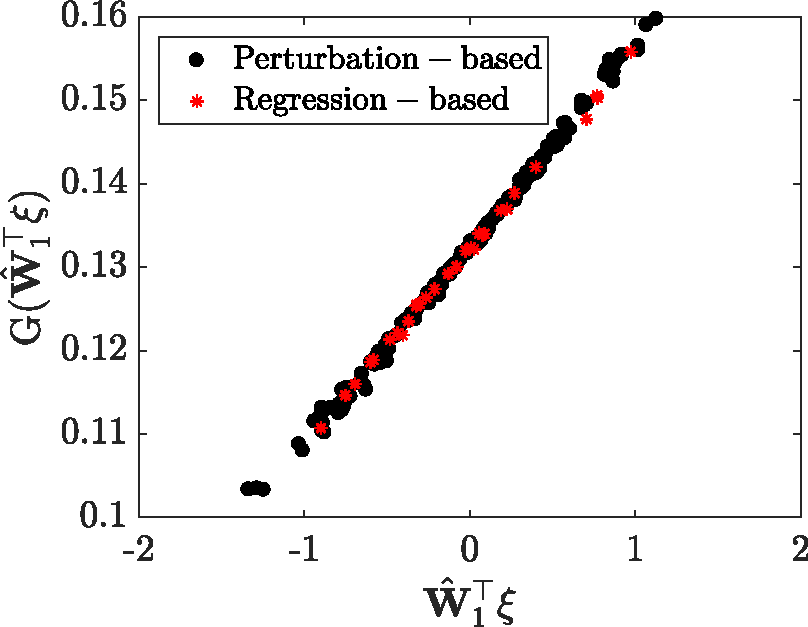
\includegraphics[width=0.48\textwidth]{./Figures/comp_ssp}
\caption{An illustrative comparison of the SSPs generated using the gradient-based and the gradient-free approaches.}
\label{fig:comp_ssp}
\end{center}
\end{figure}
%
The two SSPs are observed to be in excellent agreement with each other. Moreover, it is interesting to note
that the variability in ignition
delay based on the considered prior marginals for $A_i$'s is observed to be approximately linear in the
active subspace; consistent with the fact the it is 1-dimensional.
\alennote{The last sentence is incomplete; also clarify that ``it'' refers to 
the active subspace.} 

We complement the comparative assessment of the two approaches by estimating
the activity scores for individual uncertain parameters ($\alpha_i$) using the
components of the dominant eigenvector as shown in Algorithm~\ref{alg:grad}.
The activity scores (\alennote{relative activity scores?}) for the 19 uncertain pre-exponents ($A_i$'s), estimated
using the gradient-based and gradient-free approaches are plotted in
Figure~\ref{fig:comp_as} (left).  Additionally, for the purpose of
verification, we compare these estimates with those obtained using the
corresponding DGSMs, as reported in~\cite{Vohra:2018}, in
Figure~\ref{fig:comp_as} (right). 

%
\begin{figure}[htbp]
 \begin{center}
  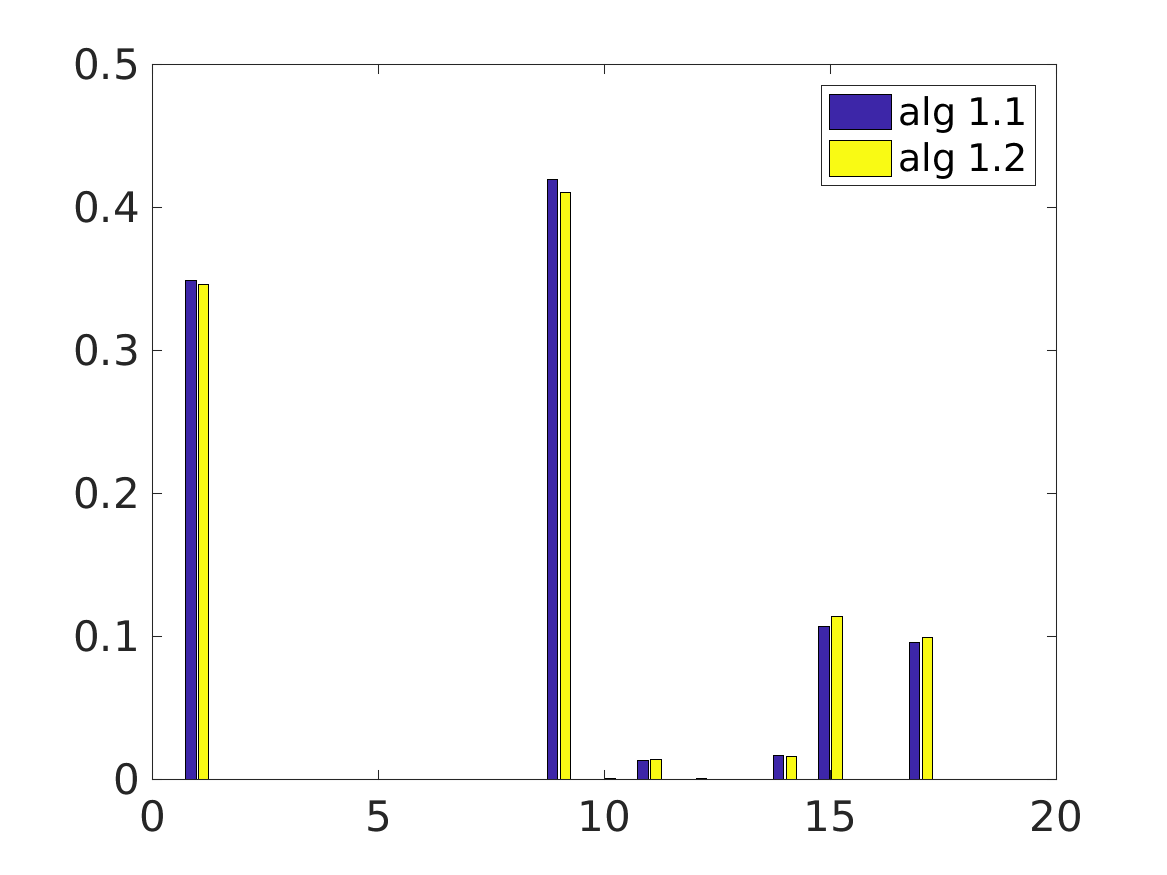
\includegraphics[width=0.45\textwidth]{./Figures/comp_as}
  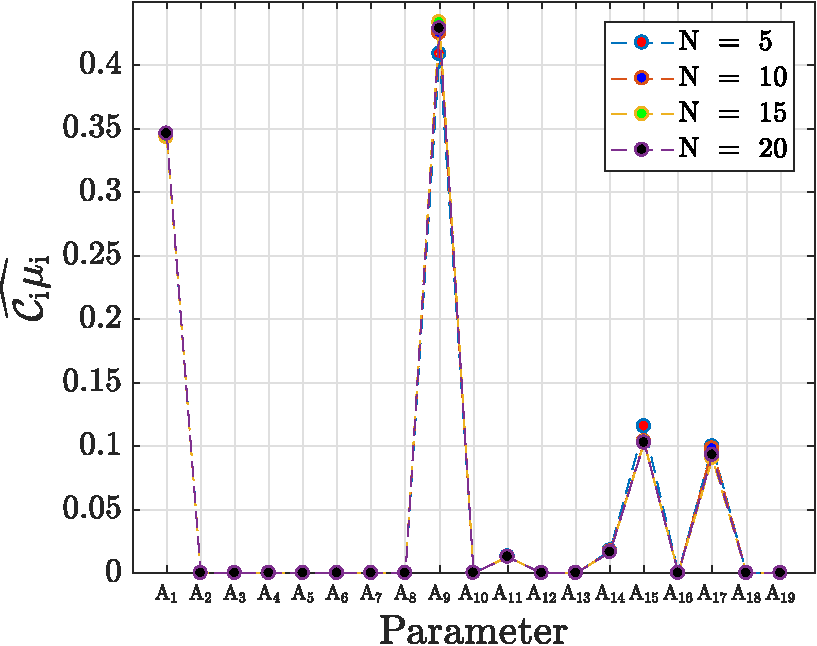
\includegraphics[width=0.45\textwidth]{./Figures/ub_conv_kinetics_rich}
\caption{Left: A bar-graph of activity scores ($\alpha_i$'s) for the 19 uncertain pre-exponents ($A_i$'s).
Right: A plot of the screening metric ($\widehat{\mathcal{C}_i\mu_i}$), defined as a normalized product of the
Poincare constant and the DGSM ($\mu_i$) (adapted from~\cite{Vohra:2018}).}
\label{fig:comp_as}
\end{center}
\end{figure}
%
The activity scores estimated using the two approaches agree favourably with each other as well as those
based on the screening metric involving the DGSMs from~\cite{Vohra:2018}. It is observed that the uncertainty
associated with the ignition delay is largely due to the uncertainty in $A_9$ and $A_1$. Sensitivity towards
$A_{15}$ and $A_{17}$ is also found to be significant. 

The above comparisons establish consistency between gradient-based and
gradient-free approaches. Due to its reduced computational overhead, the
gradient-free approach is our method of choice for the 33-dimensional problem
in the next section. 


